
\iflong
\section{Hierarchical Bayesian Content Models}
\fi

\begin{frame}{What should the content model look like?}
	\begin{itemize}
		\item Should know what kinds of questions there are
                  \begin{itemize}
                    \item Humans do the same thing
                      \item Prevents crazy wrong answers (e.g. ``entropy'' for
                        ``Brahms'' when ``Schumann'' would be better)
                    \end{itemize}
		\item Should know how questions are structured
		\begin{itemize}
			\item Titles
			\item Quotes
                          \item Relationships
		\end{itemize}
                \pause
                 \item Add bigrams and categories to Bayesian model~\cite{wood-09}
	\end{itemize}

\iflong
\else
\pause

\vspace{-4cm}

  \begin{block}{Short story:}
    \begin{itemize}
      \item Models know universe of possible categories ({\bf cat}),
    \item How questions were structured ({\bf
      bigram})
    \item Will hopefully do better than ({\bf na\"ive}) model
      \end{itemize}
    \end{block}
\fi

\end{frame}

\iflong

\begin{frame}{Richer Content Models}

\begin{enumerate*}
  \item For each category $c$ of questions, draw a distribution over words
    \alert<4>{$\theta_c \sim \dir{\lambda_1 \theta_0}$}.
    \begin{itemize*}
   \alert<3>{ \item For each label $l$ in category $c$, draw a distribution over words
      $\theta_{l,c} \sim \dir{\lambda_2 \theta_c}$ }
   \alert<2>{   \item For each type $v$, draw a bigram distribution $\theta_{l,c,v} \sim
        \dir{\lambda_3 \theta_{l,c}}$ }
  \end{itemize*}
  \item Draw a distribution over labels $\phi \sim \dir{\alpha}$.
  \item For each question with category $c$ and $N$ words, draw answer $l \sim \mult{\phi}$:
    \begin{itemize*}
\footnotesize
      \item Assume $w_0 \equiv \mbox{\textsc{Start}}$
     \alert<1>{ \item Draw $w_n \sim \mult{\theta_{l,c,w_{n-1}}}$ for $n \in \{1 \dots N\}$ }
    \end{itemize*}
\end{enumerate*}

\only<5>{
 
\vspace{-4cm}

  \begin{block}{Short story:}
    \begin{itemize}
      \item Models know universe of possible categories ({\bf cat}),
    \item How questions were structured ({\bf
      bigram})
    \item Will hopefully do better than ({\bf na\"ive}) model
      \end{itemize}
    \end{block}
}

\end{frame}

\fi

\begin{frame}{Performance with rich content models}

\begin{center}
\iflong
\begin{tabular}{ll|ccc|c}
Strategy &  Model     &	Mean&	Best&	Median&	Index\\
\hline
\multirow{4}{*}{Classify}
& na\"ive & -4.02 & -7.41 & -2.63 & 77.33 \\
& cat & -1.69 & -5.22 & 0.12 & 67.97 \\
& bigram & -3.80 & -7.66 & -2.51 & 78.69 \\
& bgrm+cat & {\bf -0.86} & {\bf -4.46} & {\bf 0.83} & 63.42 \\
\hline
\multirow{4}{*}{Oracle}
& naive & 3.36 & 0.61 & 4.35 & 49.90 \\
& cat & 4.48 & 1.64 & 5.47 & 47.88 \\
& bigram & 3.58 & 0.87 & 4.61 & 49.34 \\
& bgrm+cat & {\bf 4.67} & {\bf 1.99} & {\bf 5.74} & 46.49 \\
\hline
\end{tabular}

\else

\begin{tabular}{ll|c|c}
Strategy &  Model    &	Points &	Index\\
\hline
\multirow{4}{*}{Classify}
& na\"ive & -1.63 & 77.33 \\
& \invisible<-1>{ cat} & \invisible<-1>{ 0.12} & \invisible<-1>{ 67.97} \\
& \invisible<-2>{ bigram} & \invisible<-2>{-1.51} & \invisible<-2>{ 78.69} \\
& \invisible<-3>{ bgrm+cat} & \invisible<-3>{{\bf 0.83}} & \invisible<-3>{ 63.42} \\
\hline
\end{tabular}

\fi
\end{center}


\only<5>{

\vspace{-3cm}

\begin{block}{Beating median player}
  \begin{itemize}
    \item As far as we got (so far)
      \item But we're still not beating best players
        \item Where can we improve?
    \end{itemize}
\end{block}

}

\end{frame}

\iflong

\begin{frame}[t]

\frametitle{Error Analysis}

\begin{columns}

	\column{.4 \linewidth}
        \only<5-> {

		\begin{itemize}
			\item \alert<5> { Too slow }
			\item \alert<6> {Coreference \cite{haghighi-07} and correct question
type \cite{moldovan-00}}
			\item \alert<7> {Not enough information / not weighting later clues higher }
		\end{itemize}

}

	\column{.6 \linewidth}

		\begin{center}
			\only<1>{  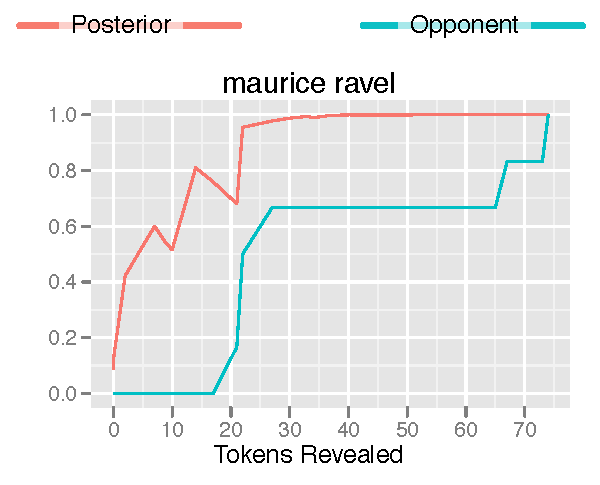
\includegraphics[width=.9\linewidth]{qb/real_question_ravel_0} \\ }
			\only<2>{  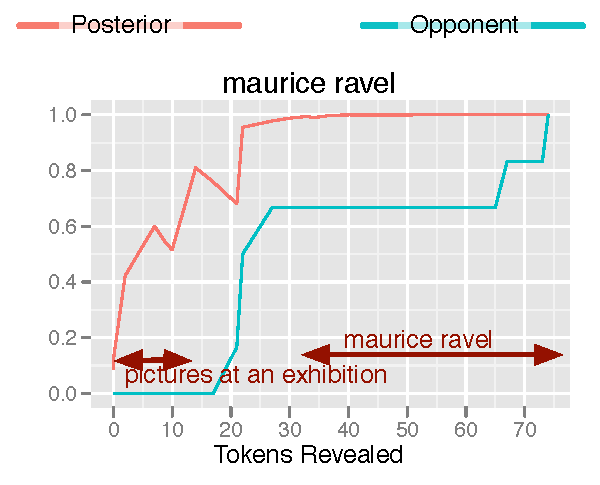
\includegraphics[width=.9\linewidth]{qb/real_question_ravel_1} \\ }
			\only<3>{  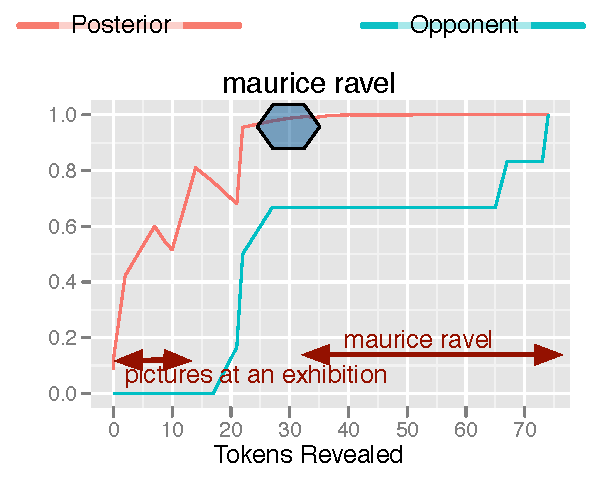
\includegraphics[width=.9\linewidth]{qb/real_question_ravel_2}
                          \\ }
			\only<4-5>{  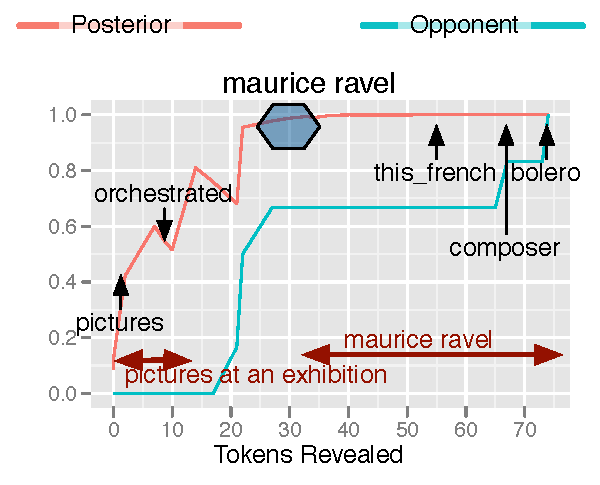
\includegraphics[width=.9\linewidth]{qb/real_question_ravel_3} \\ }
			\only<6>{  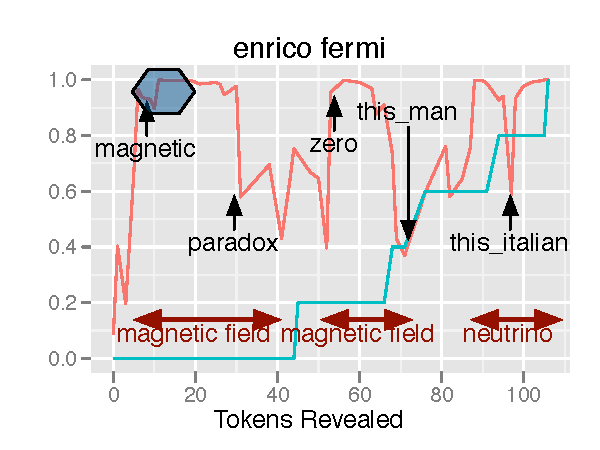
\includegraphics[width=.9\linewidth]{qb/real_question_fermi} \\ }
			\only<7>{  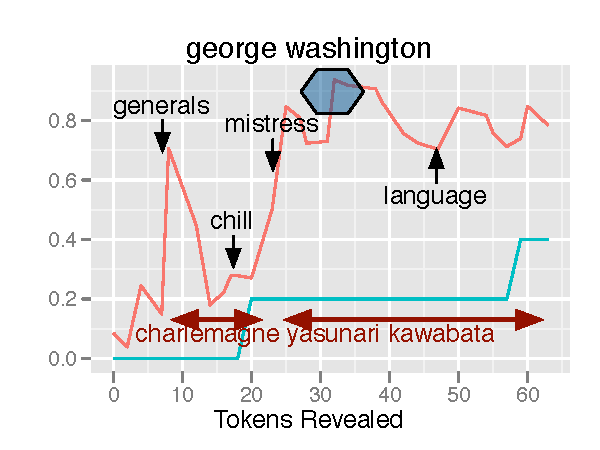
\includegraphics[width=.9\linewidth]{qb/real_question_washington} \\ }
			\only<2>{ 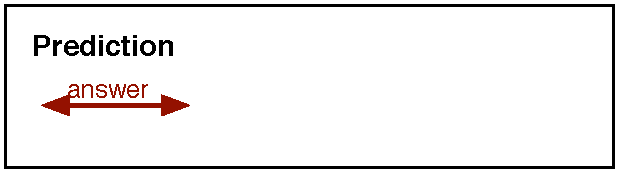
\includegraphics[width=.9\linewidth]{qb/real_question_key_0} }
			\only<3>{ 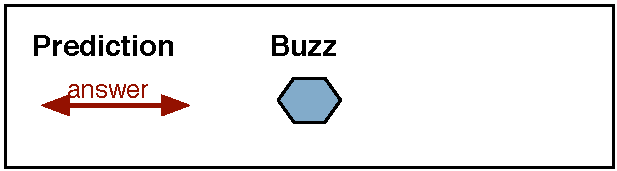
\includegraphics[width=.9\linewidth]{qb/real_question_key_1} }
			\only<4->{ 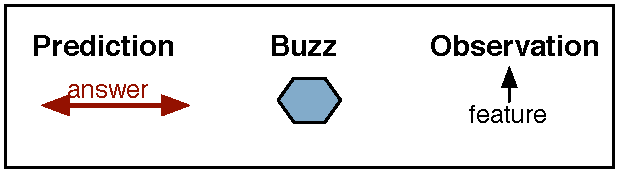
\includegraphics[width=.9\linewidth]{qb/real_question_key_2} }
		\end{center}
\end{columns}

\end{frame}

\else

\begin{frame}{Error Analysis}
  \begin{itemize}
    \item Simple stuff: Too slow
    \item Coreference \cite{haghighi-07} / question type \cite{moldovan-00}: Answering ``electric field'' for ``Enrico
      Fermi''
    \item Not enough data: Answering ``Yasunari Kawabata'' for ``George Washington''
  \end{itemize}
\end{frame}

\fi